\section{Results}
\subsection{Laser Threshold Current}

The current at which the diode transitions from emitting LED 
to laser light is determined as
\begin{equation*}
    I_\text{threshold}=\SI{35.3}{\milli\ampere}.
\end{equation*}
Figure \ref{fig:threshold} illustrates the radiation 
emitted by the diode at two current values: 
$I = \SI{35.0}{\milli\ampere}$ (see \ref{fig:a}) and 
$I = \SI{35.3}{\milli\ampere}$ (see \ref{fig:b}). 
The sharp increase in intensity corresponds to the 
onset of laser operation.

\begin{figure}
    \centering
    \begin{subfigure}{0.45\textwidth}
      \centering
      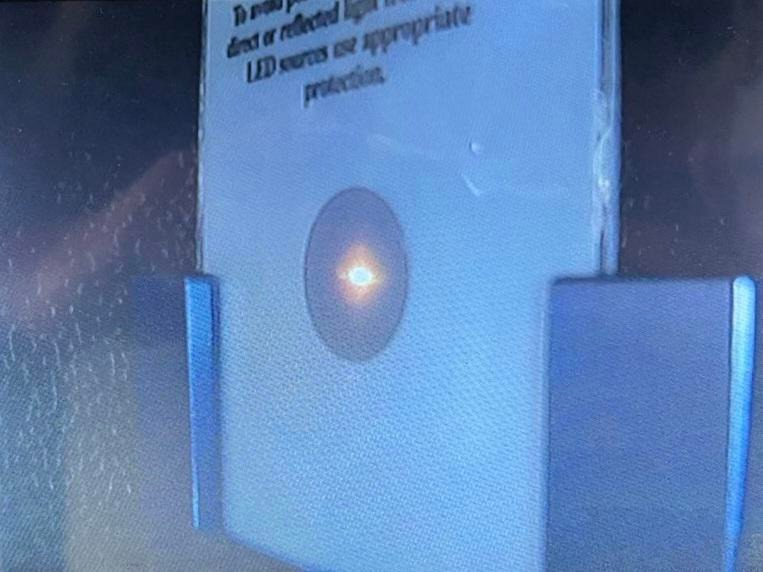
\includegraphics[width=\textwidth]{pictures/LED.jpeg}
      \caption{Diodelaser below the threshold. The diode operates as an LED.}
      \label{fig:a}
    \end{subfigure}
    \hfill
    \begin{subfigure}{0.45\textwidth}
      \centering
      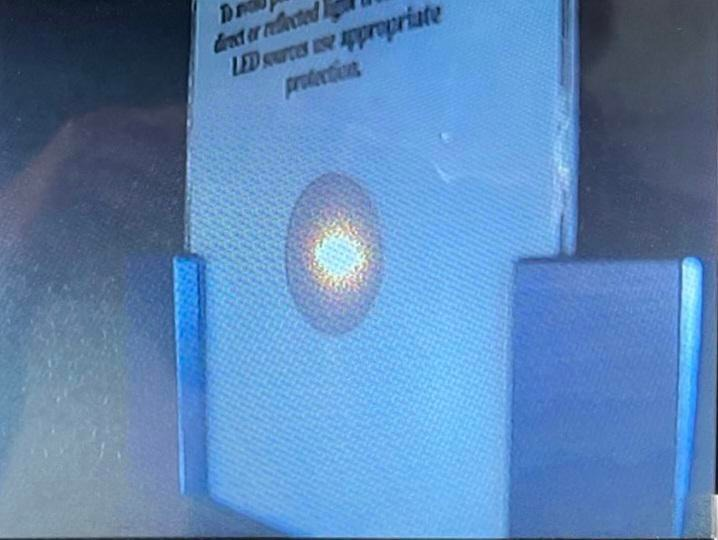
\includegraphics[width=\textwidth]{pictures/Laser.jpeg}
      \caption{Diodelaser above the threshold. The diode operates as Laser.}
      \label{fig:b}
    \end{subfigure}
    \caption{Comparison of diode operation below and above the threshold.}
    \label{fig:threshold}
\end{figure}

\subsection{Rubidium Fluorescence}
Figure \ref{fig:fluorescence} displays the fluorecence light 
emitted by rubidium. 
\begin{figure}
    \centering
    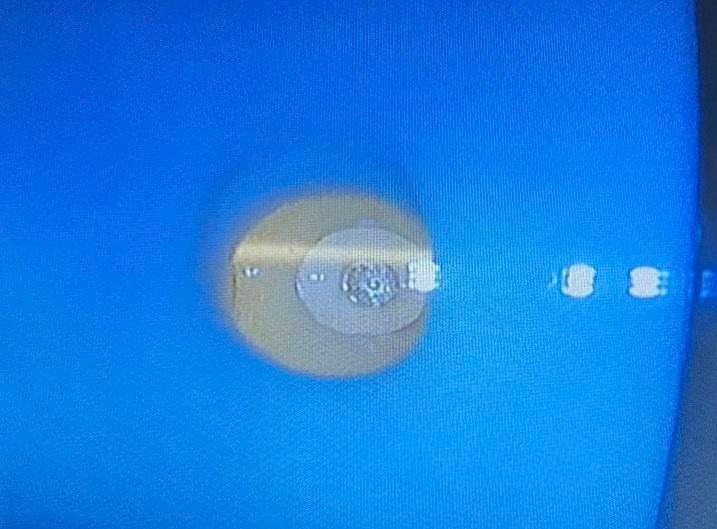
\includegraphics[width=0.5\textwidth]{pictures/Strahl.jpeg}
    \caption{Picture of the yellow fluorescence beam within the rubidium vapour.}
    \label{fig:fluorescence}
\end{figure}

\subsection{Rubidium Absorption Spectrum}
The measured absorption spectrum is depicted in Figure \ref{fig:spectrum_1}, 
while the theoretical expectation is presented in Figure \ref{fig:spectrum_2}.
\begin{figure}
    \centering
    \begin{subfigure}{0.45\textwidth}
      \centering
      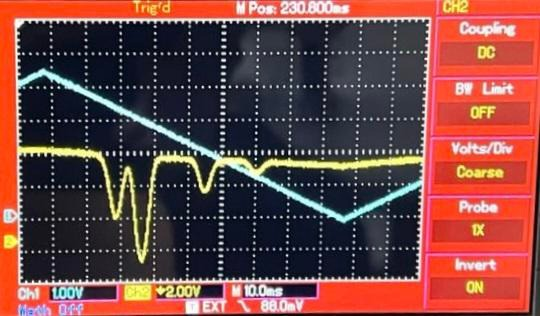
\includegraphics[width=\textwidth]{pictures/Spektrum.jpeg}
      \caption{Absorption spectrum of $^{85}\text{Rb}$ and $^{85}\text{Rb}$ (yellow) and triangular voltage of the generator (blue) as a function of time.}
      \label{fig:spectrum_1}
    \end{subfigure}
    \hfill
    \begin{subfigure}{0.45\textwidth}
      \centering
      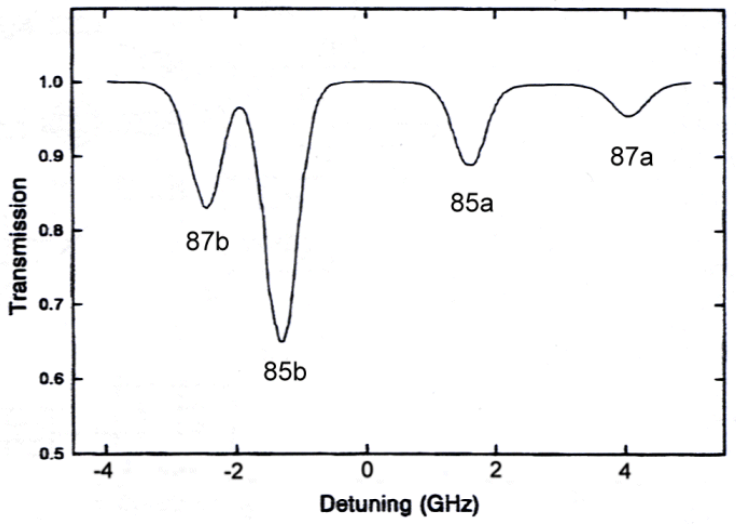
\includegraphics[width=\textwidth]{pictures/Theoriespektrum.png}
      \caption{Theoretical prediction of the absorption spectrum of $^{85}\text{Rb}$ and $^{85}\text{Rb}$. The frequency of the minima corresponds to the energy transitions in the rubidium atoms. \cite{satabs1}}
      \label{fig:spectrum_2}
    \end{subfigure}
    \caption{Rubidium absorption spectrum measurements and theoretical predictions.}
    \label{fig:spectrum}
\end{figure}
